\subsection{Cut-off and Saturation Regions:}

The circuit of Figure 3.3.0 were simulated with the {\bfseries\itshape 2N2222A} transistora and the resistors used in the laboratory, this to compare the development results with the simulated. and also, with the theoretical results in section 3.5.

{\bfseries\itshape
\begin{itemize}
\item Simulation of Cut-off and Saturation points implementing a 2N2222A transistor and a 10K $\Omega$ resistor in $R_{B}$:
\end{itemize}}

\begin{multicols}{2}
\begin{figure}[H]
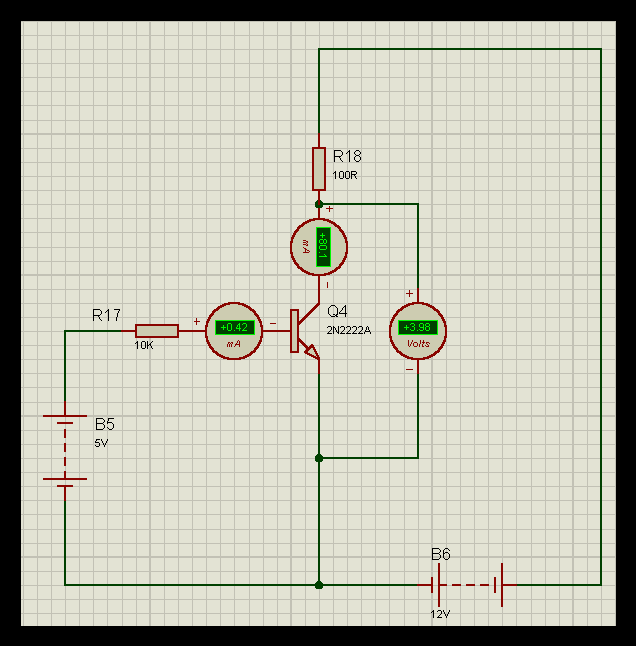
\includegraphics[width = 8cm, height = 10cm]{Cutoff-10K-5V.png}
\centering \linebreak \linebreak Figure 4.2.0: Simulated measures with a voltage source of $V_{i}$ = 5 V.
\end{figure}

\begin{figure}[H]
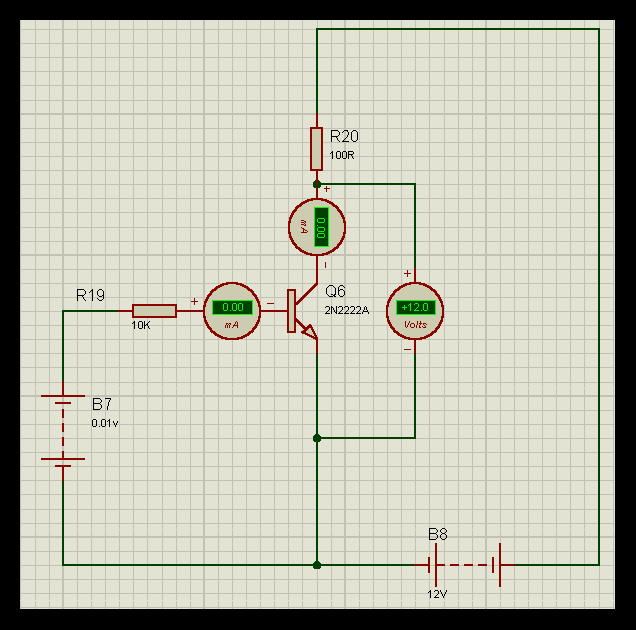
\includegraphics[width = 8cm, height = 10cm]{Cutoff-10K-0V.png}
\centering \linebreak \linebreak Figure 4.2.1: Simulated measures with a voltage source of $V_{i}$ = 0 V.
\end{figure}
\end{multicols}

\begin{center}
\begin{tabular}[.5cm]{c c c}
\toprule
\toprule
\hspace{120pt} & \hspace{50pt} {\bfseries $V_{i}$ = 5 V} \hspace{50pt} & \hspace{50pt} {\bfseries $V_{i}$ = 0 V} \hspace{50pt} \\
\midrule
\midrule
$V_{CE}$ & 3.98 V & 12 V \\
\cmidrule{1-3}
$I_{B}$ & 420 $\mu$A & 0 A \\
\cmidrule{1-3}
$I_{C}$ & 80 mA & 0 A \\
\bottomrule
\linebreak
\end{tabular}
\linebreak Table 7: $R_{C} = 100 \Omega$ and $R_{B} = 10K \Omega$ simulated measures.
\end{center}

\pagebreak

{\bfseries\itshape
\begin{itemize}
\item Simulation of Cut-off and Saturation points implementing a 2N2222A transistor and a 22K $\Omega$ resistor in $R_{B}$:
\end{itemize}}

\begin{multicols}{2}
\begin{figure}[H]
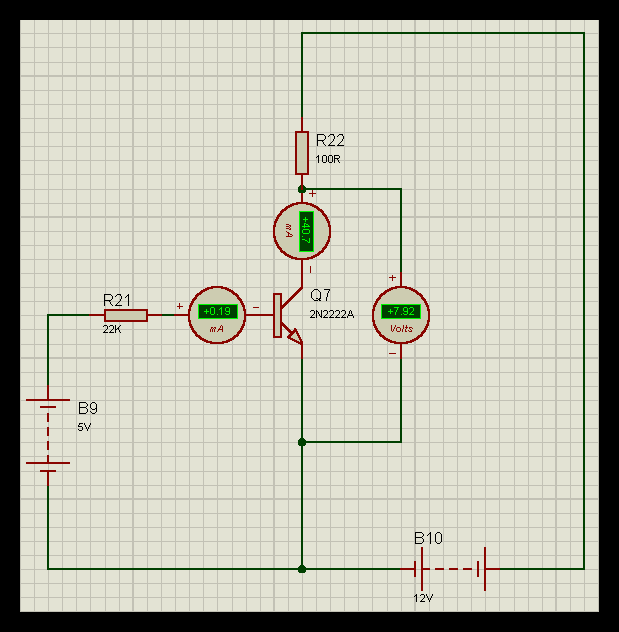
\includegraphics[width = 8cm, height = 10cm]{Cutoff-22K-5V.png}
\centering \linebreak \linebreak Figure 4.2.2: Simulated measures with a voltage source of $V_{i}$ = 5 V.
\end{figure}

\begin{figure}[H]
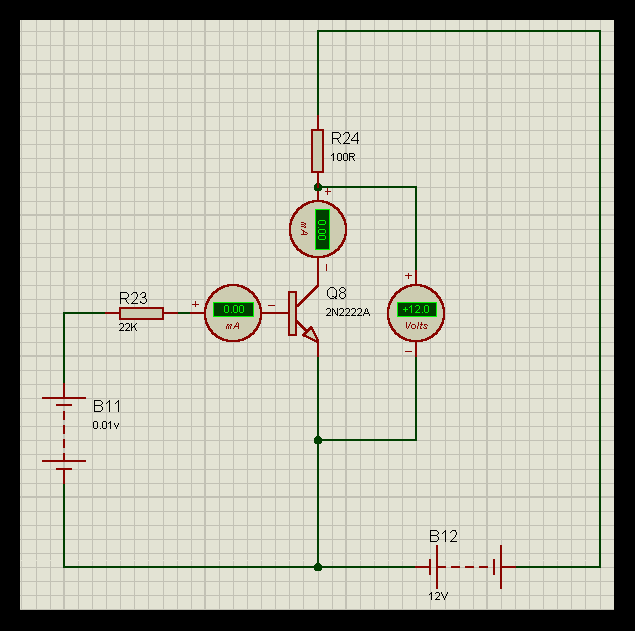
\includegraphics[width = 8cm, height = 10cm]{Cutoff-22K-0V.png}
\centering \linebreak \linebreak Figure 4.2.3: Simulated measures with a voltage source of $V_{i}$ = 0 V.
\end{figure}
\end{multicols}

\begin{center}
\begin{tabular}[.5cm]{c c c}
\toprule
\toprule
\hspace{120pt} & \hspace{50pt} {\bfseries $V_{i}$ = 5 V} \hspace{50pt} & \hspace{50pt} {\bfseries $V_{i}$ = 0 V} \hspace{50pt} \\
\midrule
\midrule
$V_{CE}$ & 7.92 V & 12 V \\
\cmidrule{1-3}
$I_{B}$ & 190 $\mu$A & 0 A \\
\cmidrule{1-3}
$I_{C}$ & 40.7 mA & 0 A \\
\bottomrule
\linebreak
\end{tabular}
\linebreak Table 8: $R_{C} = 100 \Omega$ and $R_{B} = 22K \Omega$ simulated measures.
\end{center}

\pagebreak